\documentclass[a4paper]{jpconf}
\usepackage{graphicx}
\usepackage{lmodern}
\usepackage{cite}
\usepackage{amsmath}

\bibliographystyle{iopart-num}




\begin{document}
\title{Mixed QCD-EW two-loop amplitudes for neutral current Drell-Yan production}

\author{Narayan Rana}

\address{Department of Physics, Indian Institute of Technology Kanpur, 208016 Kanpur, India
% Dipartimento di Fisica ``Aldo Pontremoli'',  University of Milano, I-20133 Milano, Italy
}

\ead{narayan@iitk.ac.in}


\begin{abstract}
We present the mixed QCD-EW two-loop virtual amplitudes for the neutral current Drell-Yan production. The evaluation of the two-loop amplitudes is one of the bottlenecks for the complete calculation of the NNLO mixed QCD-EW corrections. We present the computational details, especially the evaluation of all the relevant two-loop Feynman integrals using analytical and semi-analytical methods. We perform the subtraction of universal infrared singularities and present the numerical evaluation of the hard function.
\end{abstract}





%************
% Definition
%************

\def\D{{\cal D}}
\def\DD{\overline{\cal D}}
\def\g{\overline{\cal G}}
\def\gm{\gamma}
\def\M{{\cal M}}
\def\ep{\epsilon}
\def\epm1{\frac{1}{\epsilon}}
\def\epm2{\frac{1}{\epsilon^{2}}}
\def\epm3{\frac{1}{\epsilon^{3}}}
\def\epm4{\frac{1}{\epsilon^{4}}}
\def\unM{\hat{\cal M}}
\def\ashat{\hat{a}_{s}}
\def\asmur{a_{s}^{2}(\mu_{R}^{2})}
\def\sigbar{{{\overline {\sigma}}}\left(a_{s}(\mu_{R}^{2}), L\left(\mu_{R}^{2}, m_{H}^{2}\right)\right)}
\def\sigbarn{{{{\overline \sigma}}_{n}\left(a_{s}(\mu_{R}^{2}) L\left(\mu_{R}^{2}, m_{H}^{2}\right)\right)}}
\def\unas{ \left( \frac{\hat{a}_s}{\mu_0^{\epsilon}} S_{\epsilon} \right) }
\def\rnM{{\cal M}}
\def\bt{\beta}
\def\cD{{\cal D}}
\def\cC{{\cal C}}
\def\ca{\text{\tiny C}_\text{\tiny A}}
\def\cf{\text{\tiny C}_\text{\tiny F}}
\def\ct{{\red []}}
\def\sv{\text{SV}}
\def\murOmu{\left( \frac{\mu_{R}^{2}}{\mu^{2}} \right)}
\def\bb{b{\bar{b}}}
\def\bt0{\beta_{0}}
\def\bt1{\beta_{1}}
\def\bt2{\beta_{2}}
\def\bt3{\beta_{3}}
\def\gm0{\gamma_{0}}
\def\gm1{\gamma_{1}}
\def\gm2{\gamma_{2}}
\def\gm3{\gamma_{3}}
\def\nn{\nonumber}
\def\l{\left}
\def\r{\right}
\def\nn{\nonumber \\&}

\def\asr{\left( \frac{\alpha_s}{4 \pi} \right)}
\def\asrhat{\left( \frac{\hat\alpha_s}{4 \pi} \right)}
\def\aem{\left( \frac{\alpha}{4 \pi} \right)}
\def\uaem{\left( \frac{\hat\alpha}{4 \pi} \right)}
\def\smu{\left( \frac{s}{\mu^2} \right)}
\def\J{{\cal J}}
\def\S{{\cal S}}
\def\I{{\cal I}}

\newcommand\as{\alpha_{s}}


\newcommand{\be}{\begin{equation}}
\newcommand{\ee}{\end{equation}}
\newcommand{\bea}{\begin{eqnarray}}
\newcommand{\eea}{\end{eqnarray}}
\newcommand{\smallw}{{\scriptscriptstyle W}}
\newcommand{\mt}{m_t}
\newcommand{\ml}{m_\ell}
\newcommand{\mw}{\mu_\smallw}
\newcommand{\mwsq}{\mu_\smallw^2}
\newcommand{\mwc}{\mu_{\smallw 0}}
\newcommand{\smallz}{{\scriptscriptstyle Z}}
\newcommand{\mz}{\mu_\smallz}
\newcommand{\mzsq}{\mu_\smallz^2}
\newcommand{\mzc}{\mu_{\smallz 0}}
\newcommand{\cmz}{\bar{\mu}_{\smallz}}
\newcommand{\oa}{${\cal O}(\alpha)~$}
\newcommand{\oaa}{${\cal O}(\alpha^2)~$}
\newcommand{\oas}{${\cal O}(\alpha_s)~$}
\newcommand{\oaas}{${\cal O}(\alpha\alpha_s)~$}
\newcommand{\sineffl}{\sin\theta_{eff}^{\ell}\,}
\newcommand{\coseffl}{\cos\theta_{eff}^{\ell}\,}
\newcommand{\seffl}{\sin^2\theta_{eff}^{\ell}\,}
\newcommand{\ceffl}{\cos^2\theta_{eff}^{\ell}\,}
\newcommand{\sw}{s_\smallw\,}
\newcommand{\cw}{c_\smallw\,}
\newcommand{\swd}{s_\smallw^2\,}
\newcommand{\cwd}{c_\smallw^2\,}



\section{Introduction}
\label{sec:intro}


The Drell-Yan (DY) process \cite{Drell:1970wh} plays a central role in providing precise information 
about the gauge sector of the Standard Model (SM) and its test at quantum level.
The discovery of the $W$ and $Z$ bosons~\cite{Arnison:1983rp,Banner:1983jy,Arnison:1983mk,Bagnaia:1983zx}
was possible due to both the excellent quality data collected at the Fermilab Tevatron by the CDF and D0 experiments and at the CERN LHC by the ATLAS, CMS, and LHCb experiments, and the compatibly precise theoretical estimates. 
% 
Because of the high precision achieved by current and future hadron colliders, it is henceforth of utmost importance
to reach the similar accuracy for theoretical predictions.
% 
A small deviation in the tail of the kinematical distributions in the DY process,
which can indicate for New Physics,
may only be found after such precise measurement.
% 
Hence, the inclusion of higher-order corrections becomes mandatory in order to increase the precision of the theoretical predictions.


The next-to-leading-order~(NLO) and next-to-next-to-leading-order~(NNLO) corrections in the strong coupling constant ($\as$) 
in perturbative Quantum Chromodynamics~(QCD), were computed 
in ref.~\cite{Altarelli:1979ub} and ref.~\cite{Hamberg:1990np,Harlander:2002wh}, respectively.
% 
Recently, in a series of state-of-the-art calculations \cite{Duhr:2020seh,Duhr:2020sdp,Duhr:2021vwj},
the next-to-next-to-next-to-leading-order (N$^3$LO) QCD corrections have been obtained.
% 
The NNLO QCD computations at fully differential level have been presented in refs.~\cite{Anastasiou:2003yy,Anastasiou:2003ds,Melnikov:2006kv,Catani:2009sm,Catani:2010en}.
The first estimates of the N$^3$LO QCD fiducial cross sections for the neutral current (NC) DY have been computed in ref.~\cite{Camarda:2021ict}.
% 
% 
The threshold limit of the higher-order corrections have been discussed in \cite{Moch:2005ky,Ravindran:2005vv,Ravindran:2006cg,deFlorian:2012za,Ahmed:2014cla,Catani:2014uta,Li:2014afw,Ajjath:2020ulr}.
% 
The NLO electroweak (EW) corrections in the electromagnetic coupling constant ($\alpha$) have been computed 
in refs.~\cite{Dittmaier:2001ay,Baur:2001ze,Baur:2004ig,Arbuzov:2005dd,Zykunov:2005tc,Zykunov:2006yb,CarloniCalame:2006zq,CarloniCalame:2007cd,Arbuzov:2007db,Dittmaier:2009cr}.


The large contributions from NLO QCD and EW corrections indicate that also mixed QCD-EW effects might be potentially large.
% 
In ref.~\cite{Bernaciak:2012hj,Barze:2012tt,Barze:2013fru,Frederix:2018nkq}, the NLO QCD and EW corrections have been combined
and matched with QCD and QED Parton Showers which provide a rough estimate of the mixed QCD-EW corrections.
Hence an explicit calculation is required to find the exact mixed QCD-EW effects.
% 
A lot of efforts has been recently devoted by the theory community to that direction.
In ref.~\cite{deFlorian:2018wcj,Delto:2019ewv,Cieri:2020ikq}, the mixed QCD-QED effects have been studied 
at the inclusive and differential levels for the $Z$ boson production.
% 
The complete NNLO QCD-EW corrections for the inclusive production of an on-shell $Z$ bosons have been presented in analytical form
in refs.~\cite{Bonciani:2016wya,Bonciani:2019nuy,Bonciani:2020tvf,Bonciani:2021iis}.
The differential cross-sections for the on-shell $Z$ and $W$ production, at \oaas,
have been presented in refs.~\cite{Buccioni:2020cfi} and ~\cite{Behring:2020cqi}, respectively.
% 
Towards obtaining the full NNLO QCD-EW corrections to DY process, 
the {\it pole} approximation \cite{Denner:2019vbn} has been considered in refs.~\cite{Dittmaier:2014qza,Dittmaier:2015rxo}, 
as a first step.
% 
A partial result has been obtained in ref.~\cite{Dittmaier:2020vra} for the ${\cal O}(n_F\as \alpha)$ subset.
The mixed QCD-EW corrections to the charged-current DY process has been computed in ref.~\cite{Buonocore:2021rxx},
with the reweighted two-loop virtual corrections in the {\it pole} approximation
and the rest in exact form.
% 
The complete set of NNLO QCD-EW corrections to the NC DY process 
has been computed in ref.~\cite{Bonciani:2021zzf}, including the exact two-loop virtual contributions.
% 
The major bottleneck for these complete calculations is the two-loop virtual amplitudes. 
% 
In several publications~\cite{Bonciani:2016ypc,Heller:2019gkq,Hasan:2020vwn,Long:2021fdc},
the necessary two-loop master integrals (MIs) were computed, followed by
the computation of the two-loop helicity amplitudes for NC massless lepton pair production in ref.~\cite{Heller:2020owb}.
% 
Recently, in \cite{Armadillo:2022bgm}, an independent computation at \oaas of the two-loop amplitude for the NC DY process
has been presented considering massive leptonic final state, and thus
obtaining collinear logarithms of the lepton mass.


In this proceeding, we summarize the content of \cite{Armadillo:2022bgm}. We present the computational details
with the description of $\gamma_5$ treatment, ultraviolet (UV) renormalization and infrared (IR)
subtraction procedure. We obtain the UV renormalised IR subtracted finite remainder and we present the 
numerical evaluation.



\section{Computational details}
\label{sec:comp}
We consider two-loop mixed QCD-EW corrections to NC DY process, as given by
\begin{equation}
 q(p_1) + \bar{q}(p_2) \rightarrow l^{-}(p_3) + l^{+} (p_4) \,.
\label{eq:process}
\end{equation}
% 
The bare amplitude admits a double perturbative series expansion in the two coupling constants
\begin{equation}
 | \unM \rangle = |\unM^{(0)} \rangle + \asr |\unM^{(1,0)} \rangle + \uaem |\unM^{(0,1)} \rangle  + \asrhat \uaem |\unM^{(1,1)} \rangle + \cdots
\end{equation}
% 
The \textit{hat} denotes the bare quantities.
% 
The bare amplitudes depend on the Mandelstam variables and the masses: $m_l$ is the lepton mass, and $\mw$, $\mz$ are the complex masses
of the $W$ and $Z$ boson
% 
defined as:
\begin{equation}
\mu_V^2=M_V^2-i M_V\Gamma_V\;.
\end{equation}
The mass and decay width $M_V,\Gamma_V$ are real parameters and are the pole quantities.
% i.e. correspond to the position of the pole in the complex plane of the gauge boson propagator.
The Mandelstam variables are defined as follows:
\begin{equation}
 s = (p_1+p_2)^2, \, t = (p_1-p_3)^2, \, u = (p_2-p_3)^2 \,\, {\rm with} \,\, s+t+u=2 m_l^2 \,.
\end{equation}
The on-shell conditions of the external particles are given by
\begin{equation}
 p_1^2 = p_2^2 = 0; ~ p_3^2 = p_4^2 = m_l^2;
\end{equation}
% 


\subsection{Treatment of $\gamma_5$ in Dimensional Regularisation}
\label{sec:gamma5}


Our computation includes chiral quantities, bringing the problem of defining the inherently four-dimensional object 
$\gamma_5$ in the dimensional regularisation with arbitrary space-time dimension $d$.
% 
't Hooft and Veltman proposed in \cite{'tHooft:1972fi} to abandon the anticommutation relation of $\gamma_5$ in $d$ dimensions
\begin{equation}
 \{\gamma_\mu,\gamma_5\} = 0
\end{equation}
keeping the cyclicity of the Dirac traces.
% 
While, in refs.~\cite{Kreimer:1989ke,Korner:1991sx} Kreimer et al. kept the anticommutation relation
and abandoned the cyclicity property.
% 
The two different prescriptions yield different results for the scattering amplitudes.
However, physical observables do not depend on the choice of the $\gamma_5$ prescriptions.
% 
Recently in ref.~\cite{Heller:2020owb}, it has been checked explicitly for the NC DY process at \oaas,
that these two prescriptions produce different results for the scattering amplitudes,
but the IR subtracted hard functions are same in these two prescriptions.


In our computation, we follow the Kreimer prescriptions keeping the anticommutation relation together with 
\begin{equation}
 \gamma_5^2 = 1 \,,  ~~~ \gamma_5^{\dag} = \gamma_5
\end{equation}
and use a fixed point for the Dirac traces.
% 
For the remaining single $\gamma_5$, we perform the replacement
%
\begin{align}
  \gamma_5 = i \frac{1}{4!} \varepsilon_{\nu_1 \nu_2 \nu_3 \nu_4}
  \gamma^{\nu_1}  \gamma^{\nu_2} \gamma^{\nu_3} \gamma^{\nu_4} \,,
\end{align}
%
where, $\varepsilon^{\mu\nu\rho\sigma}$ is the Levi-Civita tensor.
% The contraction of two such tensors is given by
% %
% \begin{align}
%   \label{eqn:LeviContract}
%   \varepsilon_{\mu_1\nu_1\lambda_1\sigma_1}\,\varepsilon^{\mu_2\nu_2\lambda_2\sigma_2}=
%   {\left |
%   \begin{array}{cccc}
%     \delta_{\mu_1}^{\mu_2} &\delta_{\mu_1}^{\nu_2}&\delta_{\mu_1}^{\lambda_2} & \delta_{\mu_1}^{\sigma_2}\\
%     \delta_{\nu_1}^{\mu_2}&\delta_{\nu_1}^{\nu_2}&\delta_{\nu_1}^{\lambda_2}&\delta_{\nu_1}^{\sigma_2}\\
%     \delta_{\lambda_1}^{\mu_2}&\delta_{\lambda_1}^{\nu_2}&\delta_{\lambda_1}^{\lambda_2}&\delta_{\lambda_1}^{\sigma_2}\\
%     \delta_{\sigma_1}^{\mu_2}&\delta_{\sigma_1}^{\nu_2}&\delta_{\sigma_1}^{\lambda_2}&\delta_{\sigma_1}^{\sigma_2}
%   \end{array}
%                                                                                        \right |}
% \end{align}
% %
% and all the Lorentz indices are $d$-dimensional.


\subsection{Technical details}
\label{sec:tech}

We follow a generic procedure to compute the bare matrix elements up to two loops.
% 
The Feynman diagrams are generated using two completely independent approaches,
one based on {\tt QGRAF}~\cite{Nogueira:1991ex} and the other on {\tt FeynArts} \cite{Hahn:2000kx}.
% 
The Lorentz and Dirac algebra have been performed using 
two independent sets of in-house routines,
written in {\tt FORM} \cite{Vermaseren:2000nd} and {\tt Mathematica} \cite{Mathematica}.
The appearing scalar integrals have been reduced to the MIs by means of 
integration-by-parts (IBP) \cite{Tkachov:1981wb,Chetyrkin:1981qh} and
Lorentz invariance (LI) \cite{Gehrmann:1999as} identities,
through two independent in-house programs based on the public codes
{\sc Kira} \cite{Maierhofer:2017gsa}, {\sc LiteRed}~\cite{Lee:2013mka, Lee:2012cn} and
{\sc Reduze}2~\cite{vonManteuffel:2012np, Studerus:2009ye}.
% 
% 
To perform the reduction, it is necessary to define the integral families 
and associate each scalar Feynman integral to a specific integral family.
% As we choose to define integral families with auxiliary propagators, 
% all scalar products of a scalar Feynman integral can be expressed in terms 
% of the denominators of the particular integral family.
% 
At this point, we also consider an approximation of the scattering amplitude
to simplify our calculation.
We consider the small lepton mass limit 
i.e. $\ml$ is negligible compared
to $\mw$, $\mz$ and to the energy scales of the process.
% 
We keep only the collinear contributions from small lepton mass
which appear as $\log(\ml^2/s)$.
% 
We use this approximation in the reduction procedure,
distinguishing the integral families with $\ml$ dependence
from those where the massless lepton limit can be taken immediately.
% 
We note that the box diagrams with one or two photons exchanges,
develop these mass logarithms individually,
but they eventually cancel \cite{Frenkel:1976bj} after summing all diagrams.



The IBP reduction of all the scalar integrals to the MIs, results into the following
representation of the bare two-loop amplitudes
\begin{equation}
\langle \unM^{(0)} | \unM^{(1,1)} \rangle \, = \sum_{k=1}^{204} c_k(s,t,\{m_i\},\varepsilon) I_k(s,t,\{m_i\},\varepsilon)
\label{eq:sumint}
\end{equation}
where both the rational coefficients $c_k$ and the MIs $I_k$ depend on the dimensional regularisation parameter $\varepsilon$,
the kinematical variables $s,t$ and the masses $\{m_i\}$ of the gauge bosons and fermions.
% 
The massless two-loop form factor integrals were obtained in \cite{Gehrmann:2005pd}.
% 
By replacing top quark with the lepton, we obtain the MIs with the massive lepton 
from the planar MIs \cite{Bonciani:2008az, Bonciani:2009nb} of NNLO QCD corrections to top quark pair production.
% 
The form factor type two-loop MIs with one or two massive lines were presented in \cite{Aglietti:2003yc,Aglietti:2004tq}.
% 
The box type two-loop MIs with one and two massive lines have been computed in \cite{Bonciani:2016ypc,Heller:2019gkq,Hasan:2020vwn}.
We use the results of \cite{Bonciani:2016ypc} to obtain our MIs by relating them through the IBP identities.


The appearing 204 MIs have been computed using 
the method of differential equations \cite{Kotikov:1990kg,Remiddi:1997ny,Gehrmann:1999as,Argeri:2007up,Henn:2014qga,Ablinger:2015tua,Ablinger:2018zwz}.
% 
The solution of most of the MIs has been expressed 
in terms of generalised harmonic polylogarithms (GHPLs) \cite{Goncharov:polylog,Goncharov:2001iea,Remiddi:1999ew}.
% 
However in our results, we find 5 MIs which are not expressed,
according to ref.~\cite{Bonciani:2016ypc},
in terms of GHPLs, but using Chen-Goncharov integrals \cite{Chen:1977oja}.
% 
Although in ref.~\cite{Heller:2019gkq}, the possibility to solve these MIs in terms of Nielsen polylogarithmic functions has been discussed.
% 
It is possible to numerically evaluate the Chen iterated integrals \cite{Chen:1977oja}
in a non-physical region. However, the analytic continuation to cover the complete 
physical region, is an extremely challenging task.
% 
Hence, we adopt the following semi-analytical approach to compute particularly these 5 MIs.
% 
We consider the complete system of differential equations of the integral family which contains these 5 MIs.
We solve the whole system using series expansion method as proposed in ref.~\cite{Moriello:2019yhu}
and implemented in the {\tt Mathematica} code {\tt DiffExp} \cite{Hidding:2020ytt}.
We have written an independent implementation \cite{SeaFire} of the procedure to consistently incorporate complex masses.
% 
As we consider the complete system ($36 \times 36$) for the integral family to solve in this approach, 
the other 31 integrals are also known in terms of GHPLs.
% 
This allows us to cross-check the output of our code for these 31 MIs 
with the numerical evaluation of the analytic results in terms of GHPLs
using {\tt GiNaC} \cite{Vollinga:2004sn}. 
% 
As an additional cross-check,
we have solved the same system of differential equations
using real gauge-boson masses,
by using both {\tt DiffExp} and our private implementation, finding excellent agreement.
% 
The final results are expressed in GHPLs and of the symbols associated to these 5 MIs, which are evaluated using our code.

%
% In Figure \ref{fig:MIs} we present the real and imaginary parts
% of the values of the $\ep^0$ coefficient of the MIs numbered from 32 to 36 in ref.~\cite{Bonciani:2016ypc},
% in a phase-space region relevant for LHC phenomenology.


\subsection{Ultraviolet renormalization}

The \oaas renormalisation procedure for the NC DY production has been presented in ref.~\cite{Dittmaier:2020vra}.
We summarize here the main points.
% 
The gauge couplings and the Higgs vacuum expectation value can be expressed in terms of
the masses of the gauge bosons and the electric charge. 
% 
The on-shell electric charge counterterm at \oaa and \oaas has been presented in ref.~\cite{Degrassi:2003rw}.
The mass counterterms in the complex mass scheme \cite{Denner:2005fg} have been discussed in ref.~\cite{Dittmaier:2020vra}.
% 
The relation between the Fermi constant $G_\mu$ and the fine structure constant $\alpa$
is given by the finite correction $\Delta r$,
introduced with real gauge boson masses in ref.~\cite{Sirlin:1980nh};
its \oaas corrections were discussed in ref.~\cite{Kniehl:1989yc,Djouadi:1993ss}. 
We evaluate it here with complex-valued masses.

--------------------

The renormalised gauge boson self-energies are obtained,
by combining the unrenormalised self-energy expressions with the mass and wave function counterterms.
In the full calculation, we never introduce wave function counterterms on the internal lines,
because they would systematically cancel
against a corresponding factor stemming from the definition of the renormalised vertices.
We exploit instead the relation in the SM
between the wave function and charge counterterms \cite{Denner:2019vbn}
and we directly use the latter to define the renormalised self-energies.
% 
The expression of the two-loop Feynman integrals required for the evaluation of the
\oaas correction to the gauge boson propagators and all the needed counterterms
can be found in refs.~\cite{Kniehl:1989yc,Djouadi:1993ss,Dittmaier:2020vra}.

-----------------

\subsection{Infrared Singularities and Universal Pole Structure}
% \label{sec:infra}

The UV renormalised matrix elements still contain IR divergences
originating from soft gluons/photons and/or collinear massless partons.
% 
However, the structure of these IR divergences in the scattering amplitudes, is universal
and well-known in the case of a massless gauge theory up to two-loop level
\cite{Catani:1998bh,Sterman:2002qn,Becher:2009cu,Gardi:2009qi}.
% 
In \cite{Kilgore:2011pa,Kilgore:2013uta}, the IR structure for mixed gauge groups, 
particularly for mixed QCD$\otimes$QED corrections to NC DY production with massless leptons, 
has been studied in detail.
% 
The IR structure of the scattering amplitudes including massive particles
has also been studied in \cite{Mitov:2006xs,Becher:2007cu,Becher:2009kw,Ahmed:2017gyt,Blumlein:2018tmz}.
Recently, the IR structure of top quark pair production has been studied in detail
in \cite{Catani:2014qha} for one-loop QCD corrections
and in \cite{Catani:2019iny,Catani:2019hip,Catani:2020kkl} for two-loop level.
% 
This result can be appropriately abelianised \cite{Buonocore:2019puv} to obtain
the IR structure for the mixed QCD-EW corrections to NC DY production.


The universality of the IR divergences in the scattering amplitudes has led to the development of 
many subtraction procedures to obtain the finite remainder from the scattering amplitudes.
% 
At NLO calculations, the Catani-Seymour dipole subtraction~\cite{Catani:1996jh,Catani:1996vz,Catani:2002hc} 
and FKS subtraction~\cite{Frixione:1995ms} are the two most widely used methods.
At NNLO computations also, several techniques have been proposed (see e.g. \cite{Proceedings:2018jsb} and references therein).
% 
The subtraction of the IR poles from the matrix elements is via a process-independent subtraction operator $\mathcal{I}$.
% 
The subtraction operators within different subtraction schemes can differ from each other by a finite constant.
% 
We use here the subtraction operator which has been defined in the framework of the $q_T$-subtraction formalism~\cite{Catani:2007vq}.
% 
The one-loop IR subtraction functions ($\I$) are given by
%
\begin{align}
\I^{(1,0)} &= \smu^{-\ep} C_F \left( - \frac{2}{\ep^2} - \frac{1}{\ep} (3 + 2 i \pi)  + \zeta_2 \right) \,,
\\
%
\I^{(0,1)} &= \smu^{-\ep} \bigg[ Q_u^2 \left( - \frac{2}{\ep^2} - \frac{1}{\ep} (3 + 2 i \pi)  + \zeta_2 \right)
 + \frac{4}{\ep} {\Gamma}_{l}^{(0,1)} \bigg] \,,
\end{align}
%
where
\begin{equation}
 {\Gamma}_{l}^{(0,1)} = Q_u Q_l \log \bigg( \frac{2 p_1.p_3}{2 p_2.p_3} \bigg)
 + \frac{Q_l^2}{2} \bigg(  -1 - \frac{1+x_l^2}{1-x_l^2} \log (x_l) \bigg) \,.
\end{equation}
%
$Q_l$ and $Q_u$ are the charges of the lepton and of the initial-state quark, and the Casimir of the fundamental representation of SU(N), $C_F$, is given by $C_F=\frac{N^2-1}{2 N}$ \,.
The variable $x_l$ is given by
\begin{equation}
 \frac{(1-x_l)^2}{x_l} = -\frac{s}{\ml^2}\;.
\label{eq:defxl}
\end{equation}
% 
Using the one-loop subtraction functions, we obtain the finite contributions to
the one-loop QCD and EW amplitudes, respectively, as follows:
\begin{align}
 | \M^{(1,0),fin} \rangle &= | \M^{(1,0)} \rangle -  \I^{(1,0)} | \M^{(0)} \rangle \,,
 \label{eq:QCDfin}\\
 | \M^{(0,1),fin} \rangle &= | \M^{(0,1)} \rangle -  \I^{(0,1)} | \M^{(0)} \rangle \,.
 \label{eq:EWfin}
\end{align}
%
%
The mixed two-loop subtraction operator is given by
%%%%%%%%%%%%%%%%%%%%%%
%
\begin{align}
  \I^{(1,1)} = \smu^{-2\ep} C_F &
\bigg[
Q_u^2  \bigg( \frac{4}{\ep^4} + \frac{1}{\ep^3} ( 12 + 8 i \pi ) + \frac{1}{\ep^2} ( 9 - 28 \zeta_2 + 12 i \pi)
+ \frac{1}{\ep} \Big( -\frac{3}{2} + 6 \zeta_2
\nonumber\\&
- 24 \zeta_3 - 4 i \pi \zeta_2 \Big) \bigg)
%
+ \left( - \frac{2}{\ep^2} - \frac{1}{\ep} (3 + 2 i \pi)  + \zeta_2 \right)~\frac{4}{\ep}~\Gamma_l^{(0,1)} \bigg].
\label{eq:i11}
\end{align}
% 
Using eqs.~(\ref{eq:QCDfin}-\ref{eq:i11}), we obtain the subtracted and finite two-loop amplitude
%
\begin{equation}
  | \M^{(1,1),fin} \rangle =
  | \M^{(1,1)} \rangle -  \I^{(1,1)} | \M^{(0)} \rangle
                      - \tilde{\I}^{(0,1)} | \M^{(1,0),fin} \rangle
                      - \tilde{\I}^{(1,0)} | \M^{(0,1),fin} \rangle \,.
 \label{eq:subtracted}
\end{equation}
%
%
$\tilde{\I}^{(i,j)}$ is obtained by dropping the term proportional to $\zeta_2$ in ${\I}^{(i,j)}$.
This conventional choice defines the finite part of our subtraction term.
%



\section{Results}
\label{sec:results}
% 
Using eq.~\eqref{eq:subtracted}, we obtain the finite IR-subtracted matrix element $\langle \M^{(0)} | \M^{(1,1),fin} \rangle$
% 
\begin{align}
\langle \M^{(0)} | \M^{(1,1),fin} \rangle &= \langle \M^{(0)} | \M^{(1,1)} \rangle -  \I^{(1,1)} \langle \M^{(0)}  | \M^{(0)} \rangle
\nonumber\\&
                                                 - \tilde{\I}^{(0,1)} \langle \M^{(0)} | \M^{(1,0),fin} \rangle
                                                 - \tilde{\I}^{(1,0)} \langle \M^{(0)} | \M^{(0,1),fin} \rangle \,.
\end{align}
% 
The hard function, $H^{(1,1)}$, is  defined as
\begin{equation}
% 
 H^{(1,1)} =
 \frac{1}{16}~
\left[
  2 ~ {\rm Re} \left( \frac{\langle \M^{(0)} | \M^{(1,1),fin} \rangle}{\langle \M^{(0)} | \M^{(0)} \rangle} \right)
\right]
  \;.
\end{equation}
% 
We prepare a numerical grid for ${H}^{(1,1)}$,
covering all the phase-space values relevant for
NC DY in a given fiducial volume.
% and parameterised in terms of the partonic centre-of-mass energy $\sqrt{s}$ and scattering angle $\cos\theta$.
% 
To illustrate, we present here a grid with (130x25) points in 
the partonic centre-of-mass energy $\sqrt{s}$ and the cosine of the scattering angle $\cos\theta$,
% in  $(\sqrt{s},\cos\theta)$,
covering the intervals $s\in [40,13000]$ GeV and $\cos\theta\in [-1,1]$.
% 
Any intermediate value of ${H}^{(1,1)}$ can be extracted by interpolating the grid points.
We use the following parameters:
% 
\begin{center}
 \begin{tabular}{c l l l}
 \hline\hline
  $M_Z$ & 91.1535 GeV & $\Gamma_Z$ & 2.4943 GeV\\
  $M_W$ & 80.358 GeV  & $\Gamma_W$ & 2.084 GeV\\
  $m_H$ & 125.09 GeV  & $m_t$ & 173.07 GeV\\
 \hline\hline
 \end{tabular}
% 
\end{center}
%
We use {\tt GiNaC} and {\tt handyG} \cite{Naterop:2019xaf}
in two independent {\tt C++} and {\tt Mathematica} codes to evaluate all the GHPLs.
We also use {\tt HarmonicSums} \cite{Ablinger:2010kw,Ablinger:2014rba} and {\tt PolyLogTools} \cite{Duhr:2019tlz} for several intermediate checks.


In Figure \ref{fig:correction}, we present
\begin{figure}[t]
\begin{center}
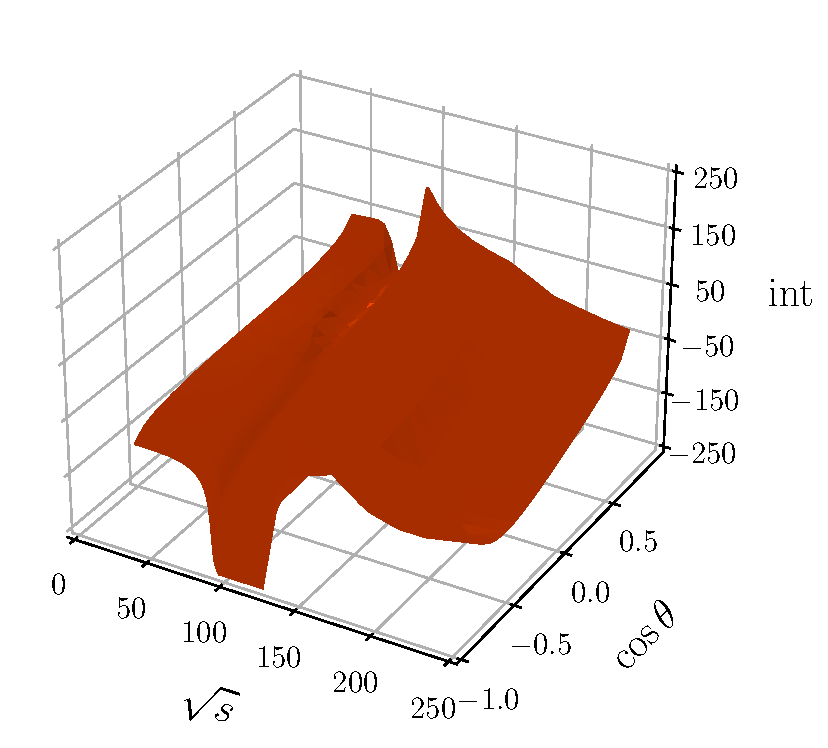
\includegraphics[width=7.5cm]{plots/correction-VB-noFSR-250.pdf}
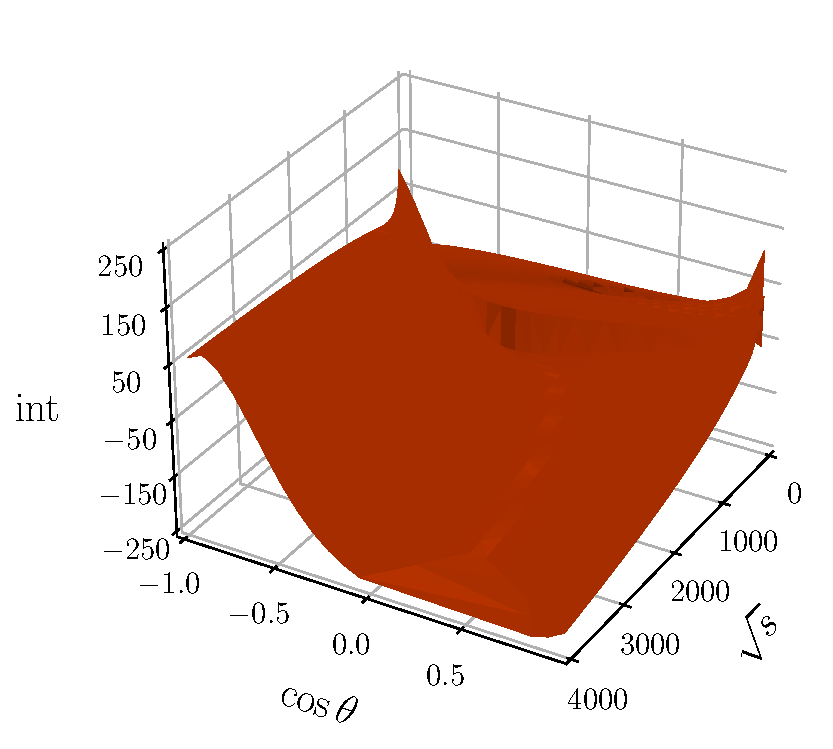
\includegraphics[width=7.5cm]{plots/correction-VB-noFSR-extended.pdf}
\end{center}
\vspace{-2ex}
\caption{\label{fig:correction}
 The contributions from all the vertex and box Feynman diagrams
 to the \oaas correction to the finite hard function,
  in two different invariant mass ranges,
  as a function of $\sqrt{s}$ and $\cos\theta$.
  }
\end{figure}
the numerical result from the UV-renormalised IR-subtracted
two-loop \oaas virtual correction due to the two-loop vertex and box Feynman diagrams.
% 
The figures show the correction normalised to the Born cross section
and expressed in units $\frac{\alpha}{\pi} \frac{\alpha_s}{\pi}$.
% as a function of $\sqrt{s}$ and $\cos\theta$.
% We consider the range $-1\leq\cos\theta\leq 1$ and,
% for the partonic center-of-mass energy, two different intervals,
% namely $50\leq\sqrt{s}\leq 250$ GeV and $50\leq\sqrt{s}\leq 5000$ GeV.

\section{Conclusions}
\label{sec:conclusions}
% 
In this proceeding, we present the content of \cite{Armadillo:2022bgm} i.e.
% 
the computational details of the \oaas virtual corrections to the NC DY production.
We summarize the technical details, followed by the UV renormalization procedure
and subtraction of the IR divergences using the subtraction operator defined 
in the framework of the $q_T$-subtraction formalism. The hard function has then 
been numerically evaluated, covering all the phase-space values relevant for NC
DY production in a given fiducial volume.




\section*{Acknowledgments}
We would like to thank T. Armadillo, R. Bonciani, S. Devoto and A. Vicini for successful collaboration. 
We would also like to thank L. Buonocore, M. Grazzini, S. Kallweit, C. Savoini and F. Tramontano for several interesting discussions.
We would like to thank G. Heinrich for help with {\sc pySecDec} and R. Lee for help with {\sc LiteRed}.
% 
N.R. is partially supported by the Italian Ministero della Universit\`a e della Ricerca (grant PRIN201719AVICI\_01).


-----------------------------------

% \begin{figure}[h]
% \begin{minipage}{14pc}
% \includegraphics[width=14pc]{name.eps}
% \caption{\label{label}Figure caption for first of two sided figures.}
% \end{minipage}\hspace{2pc}%
% \begin{minipage}{14pc}
% \includegraphics[width=14pc]{name.eps}
% \caption{\label{label}Figure caption for second of two sided figures.}
% \end{minipage} 
% \end{figure}
% 
% \begin{figure}[h]
% \includegraphics[width=14pc]{name.eps}\hspace{2pc}%
% \begin{minipage}[b]{14pc}\caption{\label{label}Figure caption for a narrow figure where the caption is put at the side of the figure.}
% \end{minipage}
% \end{figure}


\section*{References}

% \bibliography{main}
% \bibliographystyle{iopart-num}
\bibliography{iopart-num}

% \begin{thebibliography}{9}
% \bibitem{iopartnum} IOP Publishing is to grateful Mark A Caprio, Center for Theoretical Physics, Yale University, for permission to include the {\tt iopart-num} \BibTeX package (version 2.0, December 21, 2006) with  this documentation. Updates and new releases of {\tt iopart-num} can be found on \verb"www.ctan.org" (CTAN). 
% \end{thebibliography}

\end{document}


